% This is a sample LaTeX input file.  (Version of 12 August 2004.)
%
% A '%' character causes TeX to ignore all remaining text on the line,
% and is used for comments like this one.

\documentclass{article}      % Specifies the document class

\def\Course{Statistical Methods for Machine Learning}
\def\Exam{Assignment 1}
\def\Studentname{
Tudor Dragan (xlq880)\\
Nicolae Mariuta (rqt629)\\
Gabriel Carp
}
\def\Sub_date{\today}
                             % The preamble begins here.
%\title{\bf Principles of Computer Systems Design\\ {\Large Exam}}  % Declares the document's title.
%\author{Tudor Dragan\\}

\title{\textbf{\Course}\\\textbf{\Exam}}
\author{\Studentname}
\date{\Sub_date}      % Deleting this command produces today's date.

\usepackage{verbatimbox}
\usepackage{listings}
\usepackage{color}
\usepackage[]{amsmath}
\usepackage[english]{babel}
\usepackage[utf8]{inputenc}
\usepackage{graphicx}
\usepackage{moreverb}
\usepackage{hyperref}
\usepackage[T1]{fontenc} % font
\usepackage{program}
\usepackage[top=1.5in, bottom=1.5in, left=1.4in, right=1.4in]{geometry}
\usepackage[super]{nth}
\usepackage{fancyhdr}
\usepackage{lastpage}
\usepackage[linesnumbered]{algorithm2e}
\usepackage[table,xcdraw]{xcolor}
\definecolor{dkgreen}{rgb}{0,0.6,0}
\definecolor{gray}{rgb}{0.5,0.5,0.5}
\definecolor{mauve}{rgb}{0.58,0,0.82}

\lhead{\textbf{\Course}}
\rhead{\Exam~(Submission: \Sub_date)}

\cfoot{}
\lfoot{\Studentname}
\rfoot{\thepage\ of \pageref{LastPage}}
%\pagestyle{fancy}
\renewcommand{\footrulewidth}{0.4pt}


\lstset{frame=tb,
      language=Java,
      aboveskip=3mm,
      belowskip=3mm,
      showstringspaces=false,
      columns=flexible,
      basicstyle={\small\ttfamily},
      numbers=none,
      numberstyle=\tiny\color{gray},
      keywordstyle=\color{blue},
      commentstyle=\color{dkgreen},
      stringstyle=\color{mauve},
      breakatwhitespace=true
      tabsize=3
}
\newcommand{\ip}[2]{(#1, #2)}
                             % Defines \ip{arg1}{arg2} to mean
                             % (arg1, arg2).

%\newcommand{\ip}[2]{\langle #1 | #2\rangle}
                             % This is an alternative definition of
                             % \ip that is commented out.

\begin{document}             % End of preamble and beginning of text.

\maketitle                   % Produces the title.

\section*{I.2 Probability and Parameter Estimation}
\subsection*{I.2.1 Univariate Gaussian distributions}

\begin{figure}[ht]
\centering

{%
\setlength{\fboxsep}{5pt}%
\fbox{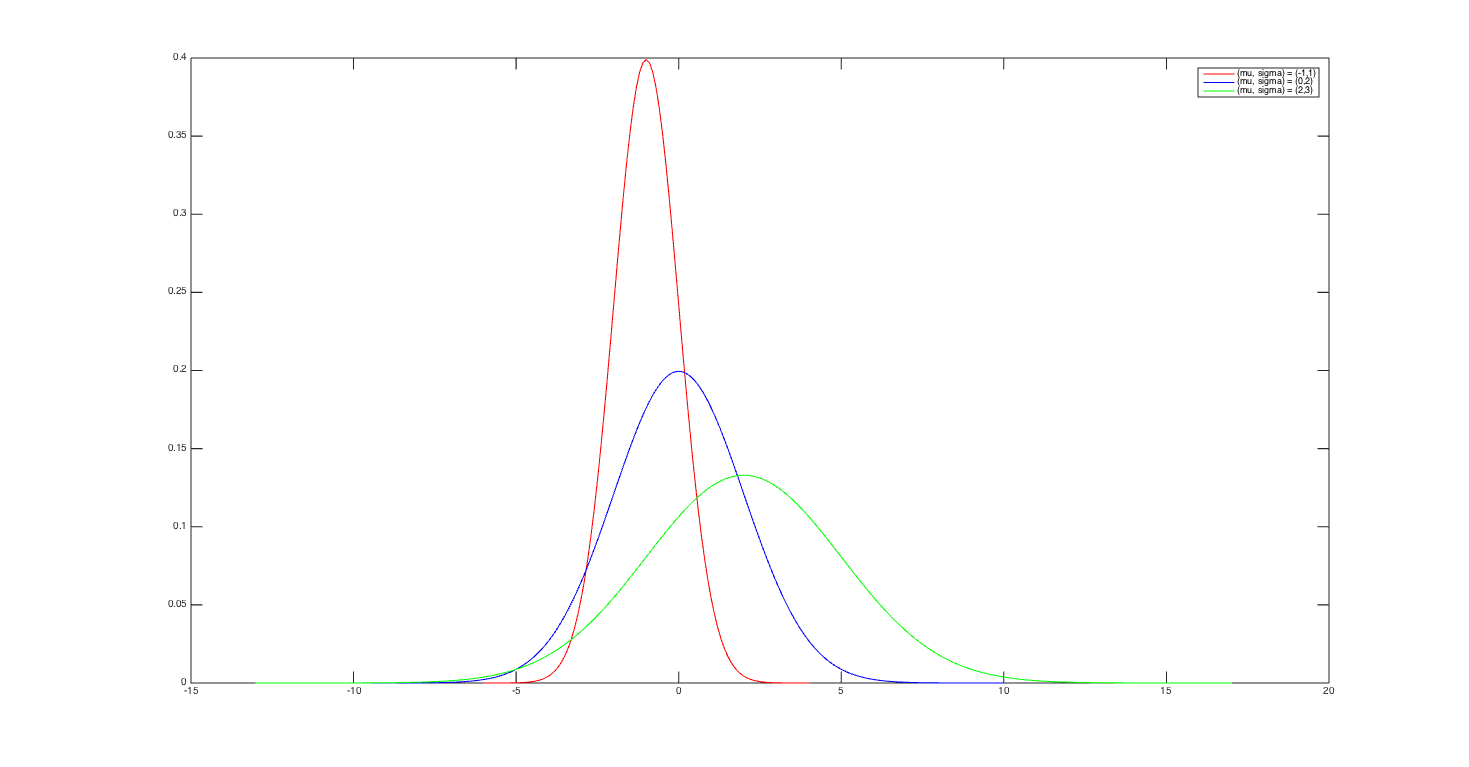
\includegraphics[scale=.3]{img/i21}}%
}%

\caption{Gaussian distribution for  \label{overflow}}
\[(\mu,\sigma) = (-1, 1), (0, 2), and (2, 3)   \]
\end{figure}

Ox in the gaussian1d function represents the input values and Oy is the output that is calculated by applying the univariate Gaussian Distribution function with means m and standard deviation d.\\

\subsection*{I.2.2 Sampling from a multivariate Gaussian distribution}

\begin{figure}[ht]
\centering

{%
\setlength{\fboxsep}{5pt}%
\fbox{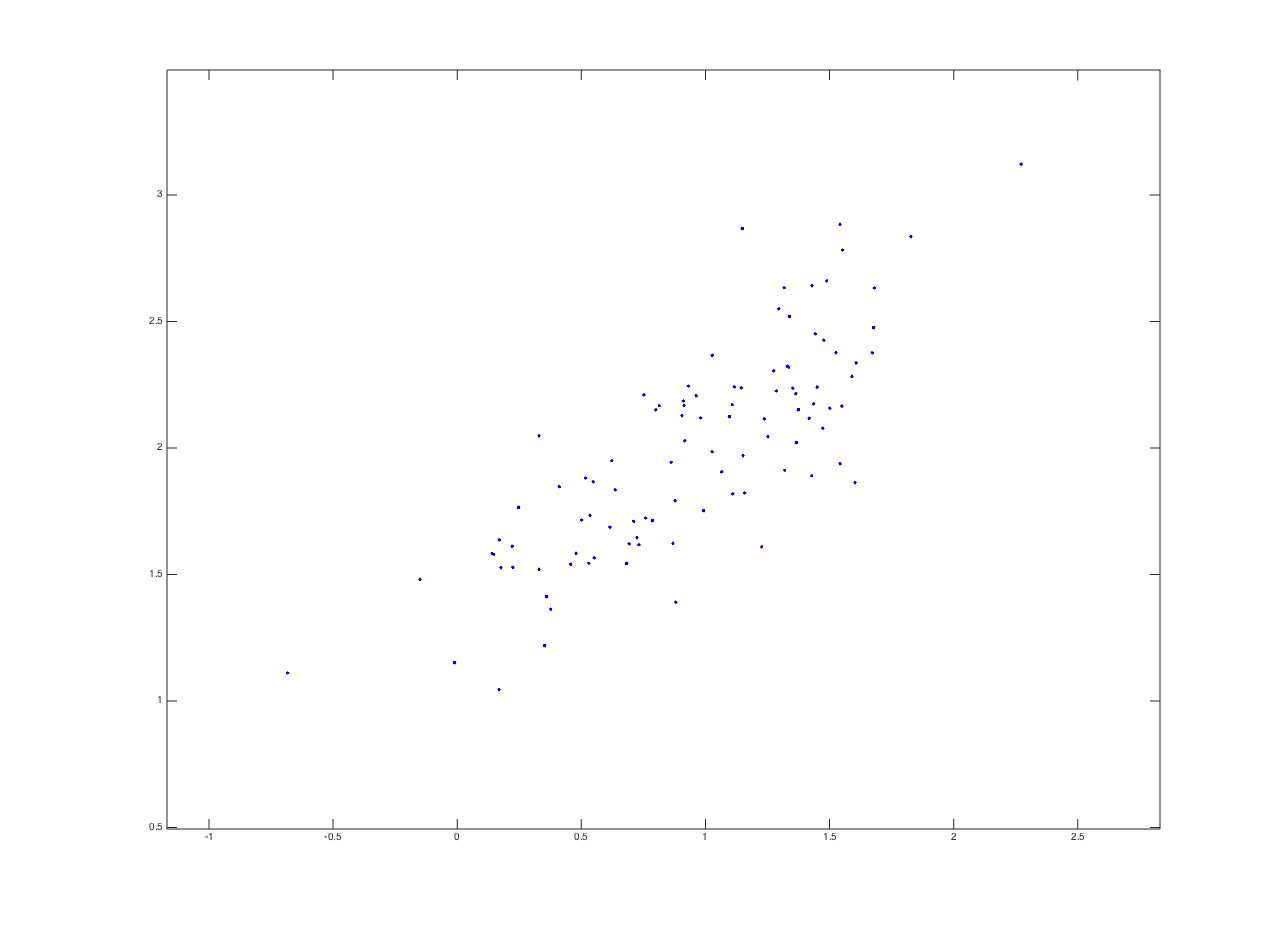
\includegraphics[scale=.3]{img/i22}}%
}%
\caption{Gaussian distribution for  \label{overflow}}
\end{figure}



\end{document}               % End of document.